% !TEX root = ../../../main.tex
% 所属：第一部分：单变量分析学 / 第3章：实数的八大基本定理
% 节：3.13 实数8大定理互证例举
% 正文按原文件顺序保存；由 ../chapter3.tex 调用。
\section{实数8大定理互证例举}
我们已经证明了8大定理的等价性，如图
\begin{center}
	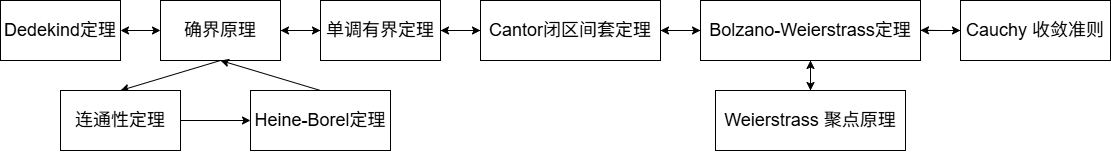
\includegraphics[width=1.0\linewidth]{figure/C2/111}
\end{center}
下面我们列举出其他的一些证明
\begin{proposition}
	用Cantor闭区间套定理证明确界原理
\end{proposition}
\begin{proof}
	
	设 $S$ 是非空有上界的实数集合，又设 $T$ 是由 $S$ 的所有上界所组成的集合，现证 $T$含有最小数，即 $S$ 有上确界．
	
	取 $a_1 \notin T, b_1 \in T$ ，显然 $a_1<b_1$ ．现按下述的规则依次构造一列闭区间：
	
	$$
	\begin{aligned}
		& {\left[a_2, b_2\right]= \begin{cases}{\left[a_1, \dfrac{a_1+b_1}{2}\right],} & \text { 若 } \dfrac{a_1+b_1}{2} \in T, \\
				{\left[\dfrac{a_1+b_1}{2}, b_1\right],} & \text { 若 } \dfrac{a_1+b_1}{2} \notin T ;\end{cases} } \\
		& {\left[a_3, b_3\right]= \begin{cases}{\left[a_2, \dfrac{a_2+b_2}{2}\right],} & \text { 若 } \dfrac{a_2+b_2}{2} \in T, \\
				{\left[\dfrac{a_2+b_2}{2}, b_2\right],} & \text { 若 } \dfrac{a_2+b_2}{2} \notin T ;\end{cases} }
	\end{aligned}
	$$
	
	$$\cdots$$
	
	由此得到一个闭区间套 $\left\{\left[a_n, b_n\right]\right\}$ ，满足
	
	$$
	a_n \notin  T, b_n \in T, \quad n=1,2,3, \cdots
	$$
	
	
	由闭区间套定理，存在惟一的实数 $\xi$ 属于所有的闭区间 $\left[a_n, b_n\right]$ ，且 $\lim\limits_{n \rightarrow \infty} a_n=\lim\limits _{n \rightarrow \infty} b_n=\xi$ ．现只需说明 $\xi$ 是集合 $T$ 的最小数，也就是集合 $S$ 的上确界．
	
	若 $\xi \notin T$ ，即 $\xi$ 不是集合 $S$ 的上界，则存在 $x \in S$ ，使得 $\xi<x$ ．由 $\lim\limits_{n \rightarrow \infty} b_n=\xi$ ，可知当 $n$ 充分大时，成立 $b_n<x$ ，这就与 $b_n \in T$ 发生矛盾，所以 $\xi \in T$ ．
	
	若存在 $\eta \in T$ ，使得 $\eta<\xi$ ，则由 $\lim\limits_{n \rightarrow \infty} a_n=\xi$ ，可知当 $n$ 充分大时，成立 $\eta<a_n$ ．由于 $a_n \in T$ ，于是存在 $y \in S$ ，使得 $\eta<a_n<y$ ，这就与 $\eta \in T$ 发生矛盾．从而得出 $\xi$ 是集合 $S$ 的上确界的结论．确界存在定理得证．
	
\end{proof}

\begin{proposition}
	确界原理证明有限覆盖定理
\end{proposition}

\begin{proof}
	构造集合 $S = \{x | a < x \leqslant b, [a, x]$ 能被 $H$ 中有限个开区间覆盖 $\}$；显然 $S$ 有上界,因 $H$ 覆盖闭区间 $[a, b]$,所以存在一个开区间 $(\alpha, \beta) \in H$ 使 $a \in (\alpha, \beta)$ .取 $x \in (\alpha, \beta)$ ,则 $[a, x]$ 能被 $H$ 中有限个开区间覆盖,从而 $x \in S$ ,故 $S$ 非空；

由确界原理存在 $\xi = \sup S$ ,现证 $\xi = b$ .用反证法.若 $\xi \neq b$ ,则 $a < \xi < b$ ,由 $H$ 覆盖闭区间 $[a, b]$,一定存在 $(\alpha_1, \beta_1) \in H$,使 $\xi \in (\alpha_1, \beta_1)$ .取 $x_1, x_2$ 使 $\alpha_1 < x_1 < \xi < x_2 < \beta_1$ ,且 $x_1 \in S$ ,则 $[a, x_1]$ 能被 $H$ 中有限个开区间覆盖,把 $(\alpha_1, \beta_1)$ 加进去,就推得 $x_2 \in S$ 这与 $\xi = \sup S$ 矛盾,故 $\xi = b$ ,即定理结论成立.
\end{proof}

\begin{proposition}
	确界原理证明$Cauchy$收敛准则
\end{proposition}
\begin{proof}
	必要性是由数列收敛定义直接得到的,不需要用到其它完备性定理.下面证充分性.（后面用其他定理证明$Cauchy$收敛准则都只证充分性,不再赘叙）
	
	设 $\{x_n\}$ 是$Cauchy$列,则 $\{x_n\}$ 是有界的（这一条也与其它实数完备性定理无关,后面用其他定理证明$Cauchy$收敛准则时直接使用,不再赘叙,请读者参考教材补充完整）.定义集合
	
	$$A = \{x | \text{存在正整数} N, \text{使任意的} n > N, \text{有} x_n > x\}  $$
	
	显然对于任意取定的 $\varepsilon > 0$ 和某个充分大的 $m$,必有 $x_m - \varepsilon \in A$,$x_m + \varepsilon \notin A$（否则将推出 $\{x_n\}$ 无界）,所以 $A$ 非空且有上界.由确界原理,$A$ 有上确界,记 $\sup A = a$.我们证明 $\{a_n\}$ 收敛于 $a$.
	
	任给 $\varepsilon > 0$,因为 $a$ 是 $A$ 的确界,故 $a - \varepsilon$ 必不是 $A$ 的上界,即存在 $x$ 属于 $A$,有 $x > a - \varepsilon$,由 $A$ 的定义知存在 $N$,使得对于任意 $n > N$,有 $x_n > a - \varepsilon$；又由$Cauchy$列的定义,存在 $N'$,使得对于任意的 $n, m > N'$,有 $|x_n - x_m| < \dfrac{\varepsilon}{2}$.显然 $a + \dfrac{\varepsilon}{2}$ 不属于 $A$,故对于 $N'$,必存在 $m' > N'$,且 $x_m \leqslant a + \dfrac{\varepsilon}{2}$,$|x_n - x_{m'}| < \dfrac{\varepsilon}{2}$,故 $x_n < a + \varepsilon$.于是任给 $\varepsilon > 0$,当 $n > \max\{N, N'\}$ 时,总有 $|x_n - a| < \varepsilon$,这就证明了$Cauchy$序列必定是收敛的.
\end{proof}
\begin{proposition}
	单调有界定理证明致密性定理
\end{proposition}
\begin{proof}
	
设 $S$ 是一有界无限点集,则在 $S$ 中可选取可数多个互不相同的点组成数列 $\{a_n\}$,显然数列 $\{a_n\}$ 是有界的.下面我们从 $\{a_n\}$ 中抽取一个单调子列,从而由单调有界定理该子列收敛,最后我们证明该子列的极限值,就是有界无限点集 $S$ 的聚点.

分两种情况来讨论：$(1)$ 如果在 $\{a_n\}$ 的任意一项之后,总存在最大的项,设 $a_1$ 后的最大项是 $a_{n_1}$,而 $a_{n_1}$ 后的最大项是 $a_{n_2}$,则显然 $a_{n_2} \leqslant a_{n_1}$.一般地,$a_{n_k}$ 后的最大项记为 $a_{n_{k+1}} (\leqslant a_{n_k}, k = 1, 2, \cdots)$.这样,就得到了 $\{a_n\}$ 的一个单调递减的子列 $\{a_{n_k}\}$,因为 $\{a_n\}$ 有界,由单调有界定理知,$\{a_{n_k}\}$ 收敛.

$(2)$. 如果 $(1)$ 不成立, 即从某一项以后, 任何一项都不是最大的, 由于前有限项不影响结果, 不妨设从第一项起, 每一项都不是最大项. 于是, 取 $a_{n_1} = a_1$ , 因 $a_{n_1}$ 不是最大项, 所以还存在另一项 $a_{n_2} > a_{n_1} (n_2 > n_1)$ , 又因为 $a_{n_2}$ 也不是最大项, 所以又有$a_{n_3} > a_{n_2} (n_3 > n_2)$ 这样一直作下去,就得到 $\{a_n\}$ 的一个单调递增子列 $\{a_{n_k}\}$,且这个子列有上界,由单调有界定理知,$\{a_{n_k}\}$ 收敛.

总之,不论 $\{a_n\}$ 属于情形 $(1)$ 还是情形 $(2)$,都可作出 $\{a_n\}$ 的一个单调收敛的子列.
\end{proof}




\begin{proposition}
	区间套定理证明确界原理
\end{proposition}

\begin{proof}
	只证明非空有上界的数集 $S$ 必有上确界,有下界的数集类似可证.

取 $S$ 的上界为 $b$ ,且 $b \notin S$ ；取 $a \in S$ ,且 $a$ 不是 $S$ 的上界,则 $a < b$ .

设闭区间 $[a_1, b_1] = [a, b]$. 

$Step\ 1$：取 $[a_1, b_1]$ 的中点 $\dfrac{a_1 + b_1}{2}$,若其是数集 $S$ 的上界,则取 $[a_2, b_2] = \left[a_1, \dfrac{a_1 + b_1}{2}\right]$；若不是数集 $S$ 的上界,则取 $[a_2, b_2] = \left[\dfrac{a_1 + b_1}{2}, b_1\right]$.

$Step\ 2$：取 $[a_2, b_2]$ 的中点 $\dfrac{a_2 + b_2}{2}$,若其是数集 $S$ 的上界,则取 $[a_3, b_3] = \left[a_2, \dfrac{a_2 + b_2}{2}\right]$；若不是数集 $S$ 的上界,则取 $[a_3, b_3] = \left[\dfrac{a_2 + b_2}{2}, b_2\right]$.

以此类推,

$Step\ n$：取 $[a_n, b_n]$ 的中点 $\dfrac{a_n + b_n}{2}$,若其是数集 $S$ 的上界,则取 $[a_{n+1}, b_{n+1}] = \left[a_n, \dfrac{a_n + b_n}{2}\right]$；若不是数集 $S$ 的上界,则取 $[a_{n+1}, b_{n+1}] = \left[\dfrac{a_n + b_n}{2}, b_n\right]$.

无限进行下去,易知

$$\lim\limits_{n \to \infty} (b_n - a_n) = \lim_{n \to \infty} \frac{b - a}{2^n} = 0. $$

(注意上述极限是$Archimedes$性质的一个等价命题) 则满足区间套定理,于是存在 $\xi \in \mathbb{R}$,有 $\xi \in \bigcap_{i=1}^{\infty} [a_i, b_i]$,且

$$\lim_{n \to \infty} b_n = \lim_{n \to \infty} a_n = \xi. $$

任取 $x \in S$ ,由二分法知 $x \leqslant b_n$ ,从而 $x \leqslant \lim\limits_{n \to \infty} b = \xi$ ,即 $\xi$ 是数集 $S$ 的一个上界.又由 $\lim\limits_{n \to \infty} a_n = \xi$ 知,$\forall \varepsilon > 0$,存在 $N$ ,当 $n > N$ 时,有 $a_n > \xi - \varepsilon$ .由分法知 $a_n$ 或者刚好是 $S$ 的上确界,或者不是 $S$ 的上界,则当 $n > N$ 时,存在 $x_0 \in S$ ,使得 $\xi - \varepsilon < a_n \leqslant x_0$.即 $\xi = \sup S$.
\end{proof}
\begin{proposition}
	区间套定理证明有限覆盖定理
\end{proposition}

\begin{proof}
	用反证法.假设定理的结论不成立,即不能用 $H$ 中有限个开区间来覆盖 $[a, b]$.

将 $[a, b]$ 等分为两个子区间,则其中至少有一个子区间不能用 $H$ 中有限个开区间来覆盖.记这个子区间为 $[a_1, b_1]$,则 $[a_1, b_1]\subset[a, b]$,且 $b_1-a_1=\dfrac{1}{2}(b-a)$.

再将 $[a_1, b_1]$ 等分为两个子区间,同样,其中至少有一个子区间不能用 $H$ 中有限个开区间来覆盖.记这个子区间为 $[a_2, b_2]$,则 $[a_2, b_2]\subset[a_1, b_1]$,且 $b_2-a_2=\dfrac{1}{2^2}(b-a)$.

重复上述步骤并不断地进行下去,则得到一个闭区间列 $\{[a_n, b_n]\}$,它满足

$$[a_n, b_n]\supset[a_{n+1}, b_{n+1}], n=1,2,\cdots, $$ $$b_n-a_n=\dfrac{b-a}{2^n}\to0(n\to\infty), $$

即 $\{[a_n, b_n]\}$ 是区间套,且其中每一个闭区间都不能用 $H$ 中有限个开区间来覆盖.

由区间套定理,存在唯一的一点 $\xi\in[a_n, b_n]$,$n=1,2,\cdots$.由于 $H$ 是 $[a, b]$ 的一个开覆盖,故存在开区间 $(\alpha, \beta)\in H$,使 $\xi\in(\alpha, \beta)$.于是,当 $n$ 充分大时有

$$[a_n, b_n]\subset(\alpha, \beta). $$

这表明 $[a_n, b_n]$ 只需用 $H$ 中的一个开区间 $(\alpha, \beta)$ 就能覆盖,与挑选 $[a_n, b_n]$ 时的假设“不能用 $H$ 中有限个开区间来覆盖”相矛盾.从而证得必存在属于 $H$ 的有限个开区间能覆盖$[a, b]$.

\end{proof}


\begin{proposition}
有限覆盖定理证明区间套定理
\end{proposition}

\begin{proof}
	反证法. 假设 $[a_n, b_n](n = 1, 2, \cdots)$ 没有公共点, 则 $[a_1, b_1]$ 上的任何一点都不是 $\{[a_n, b_n]\}$ 的公共点, 从而总存在一个开区间 $(x - \delta_x, x + \delta_x)$, 使得 $(x - \delta_x, x + \delta_x)$ 并非与所有的 $[a_n, b_n]$ 相交, 即存在 $[a_{n_x}, b_{n_x}]$, 使得 $[a_{n_x}, b_{n_x}]$ ∩ $(x - \delta_x, x + \delta_x) = \phi$.

现让 $x$ 取遍 $[a_1, b_1]$ 上的所有点就得到一个开区间集:

$$H = \{(x - \delta_x, x + \delta_x) | x \in [a_1, b_1]\}  $$

由有限覆盖定理, 可选出有限个开区间:

$$H' = \{(x_{k} - \delta_{x_k}, x_{k} + \delta_{x_k}) | k = 1, 2, \cdots, m\}  $$

覆盖闭区间 $[a, b]$, 其中

$$(x_{k} - \delta_{x_k}, x_{k} + \delta_{x_k}) \cap [a_{n_{x_k}}, b_{n_{x_k}}] = \phi  $$

因为 $[a_{n_{x_k}}, b_{n_{x_k}}]$ 只有有限个, 由区间套定理的条件, 它们是一个包含着一个, 因此其中一定有一个最小区间, 设为 $[a_{n_0}, b_{n_0}]$, 这时,

$$[a_{n_0}, b_{n_0}] \cap (x_{k} - \delta_{x_k}, x_{k} + \delta_{x_k}) = \phi, k = 1, 2, \cdots, m $$

从而,

$$[a_{n_0}, b_{n_0}] \cap \bigcup_{k=1}^{n} (x_{k} - \delta_{x_k}, x_{k} + \delta_{x_k}) = \phi $$

这就与 $[a_{n_0}, b_{n_0}] \subset [a_1, b_1]$ 矛盾. 所以 $[a_n, b_n](n = 1, 2, \cdots)$ 应有公共点.

\end{proof}
\begin{proposition}
	有限覆盖定理证明$Cauchy$收敛准则
\end{proposition}

\begin{proof}
	反证法.假设$Cauchy$列 ${x_n}$ 不收敛.已知 ${x_n}$ 为有界数列,而且 ${x_n}$ 是无穷点集（若 ${x_n}$ 是有限集,显然是收敛的）.

即存在闭区间 $[a, b]$ 使得 $\{x_n\} \subset [a, b]$. 则 $\forall x \in [a, b]$, $\exists U(x), \delta$ 使得 $U(x, \delta)$ 中只含有 $\{x_n\}$ 中的有限多项 (否则, 若 $\forall \delta > 0, U(x, \delta)$ 都有 $\{x_n\}$ 中的无限多项, 则易证 $\{x_n\}$ 收敛, 这与假设矛盾).

从而得 $[a, b]$ 的一个开覆盖 $H = \{U(x, \delta) | x \in [a, b]\}$, 由有限覆盖定理, 存在 $H$ 的一个有限子覆盖

$$H' = \{U(x_i, \delta_i) | x_i \in [a, b], i = 1, 2, \cdots, k\}, $$

所以 $\bigcup_{i=1}^{k} U(x_i, \delta_i)$ 只含有 $\{x_n\}$ 中的有限多个点, 这显然与 $\bigcup_{i=1}^{k} U(x_i, \delta_i) \supset [a, b] \supset \{x_n\}$ 矛盾. 因此 $\{x_n\}$ 必收敛.

\end{proof}


\begin{proposition}
	聚点定理证明确界原理
\end{proposition}

\begin{proof}
	设 $S$ 是非空有上界的数集.有限集时显然有上确界,不妨假设 $S$ 是无穷集合.

又设 $M$ 是 $S$ 的一个上界,如果 $M \in S$ 或者 $M$ 是 $S$ 的聚点（如果 $S$ 有聚点的话）,则 $M = \sup S$ ,定理成立.因此,下面假设 $M \in S$ 且 $M$ 不是 $S$ 的聚点.

在 $S$ 中任取一 $x_0$ ,总有 $x_0 < M$ ,考虑区间 $[x_0, M]$：

或者 $[x_0, M]$ 上只有 $S$ 的有限多个点,这时定理显然成立；或者 $[x_0, M]$ 上有 $S$ 的无穷多个点,那么, $S$ 在 $[x_0, M]$ 上的无穷多个点组成一有界的无穷点集.根据聚点原理, $S$ 在 $[x_0, M]$ 上必有聚点.

$(1)$ 若 $S$ 在 $[x_0, M]$ 上的聚点唯一,定理一定成立

事实上,若这个唯一聚点是 $x_0$ ,任取一个 $x_1 \in [x_0, M] \cap S$ ,则在 $[x_0, M]$ 上只能有 $S$ 的有限多个点（否则, $S$ 在 $[x_0, M]$ 上还有聚点,这与 $S$ 在 $[x_0, M]$ 上的聚点唯一相矛盾）,这时定理成立；

若这个唯一聚点是 $[x_0, M]$ 的内点 $\xi$ ,要么 $\xi$ 点的右边没有 $S$ 中的点,这时 $\xi = \sup S$ ,要么 $\xi$ 点右边还有 $S$ 中的点 $x_2$ ,那么在 $[x_2, M]$ 上只能有 $S$ 的有限多个点,其中最大者就是 $\sup S$ ,定理成立.

$(2)$ 若 $S$ 在 $(x_0, M)$ 上的聚点不是唯一的.

先证明下列结论成立：在 $(x_0, M)$ 内总存在一点 $x$ ,使得 $S$ 在 $[x, M]$ 上的聚点有且仅有一个.

假定这个结论不成立,那就是说对 $(x_0, M)$ 内的任意一点 $x$,或者在 $[x, M]$ 上总没有 $S$ 的聚点,或者在 $[x, M]$ 上总有 $S$ 的多个聚点.

如果前种情况发生,则根据 $x \in (x_0, M)$ 的任意性知 $(x_0, M)$ 内的任何内点都不是 $S$ 的聚点（因为假定有 $\xi \in [x_0, M]$ 是 $S$ 的聚点,则总有 $x_0 < x' < \xi < M$,于是 $[x', M]$ 上就有 $S$ 的聚点,这与在 $[x_0, M]$ 内的任意一点 $x$,$[x, M]$ 上总没有 $S$ 的聚点相矛盾）.与 $S$ 在 $(x_0, M)$ 上的聚点不是唯一的前提相矛盾.

如果后种情况发生,根据r的任意性推知$M$必是$S$的聚点,这又与前面“$M$不是$S$的聚点”的假设相矛盾.所以,上述结论必成立.

既然在 $(x_0, M)$ 内总存在一点 $x$,使得 $S$ 在 $[x, M]$ 上的聚点唯一,那么根据前面的讨论,定理成立.
\end{proof}

\begin{proposition}
	致密性定理证明有限覆盖定理
\end{proposition}

\begin{proof}
	设 $H$ 为 $[a, b]$ 的一个开覆盖,假设 $H$ 不存在有限子覆盖,则对 $[a, b]$ 二等分作区间套 $\{[a_n, b_n]\}$,使得每个 $[a_n, b_n]$ 都不存在有限子覆盖.

根据闭区间套的做法知,$\{b_n\}$ 为有界数列,故由致密性定理知,存在 $\{b_n\}$ 的子数列 $\{b_{n_k}\}$ 收敛,设 $\lim_{k \to \infty} b_{n_k} = \xi$,由 $\lim\limits_{k \to \infty} (b_{n_k} - a_{n_k}) = 0$ 知 $\lim\limits_{k \to \infty} a_{n_k} = \xi$,显然 $\xi \in [a, b]$.

由 $[a, b]$ 被 $H$ 覆盖知,存在开区间 $(\alpha, \beta) \in H$,使 $\xi \in (\alpha, \beta)$,由 $\lim_{k \to \infty} a_{n_k} = \lim\limits_{k \to \infty} b_{n_k} = \xi$ 知,存在充分大的 $K$ 使得 $[a_{n_K}, b_{n_K}] \subset (\alpha, \beta)$,这与 $[a_{n_K}, b_{n_K}]$ 不能被 $H$ 有限覆盖矛盾.故 $H$ 必有有限子覆盖.
\end{proof}


\begin{proposition}
	 $Cauchy$ 收敛准则证明单调有界定理
\end{proposition}

\begin{proof}
	设 $\{x_n\}$ 为递增有上界数列,下面我们用反证法证明数列 $\{x_n\}$ 有极限.假设 $\{x_n\}$ 不存在极限.由$Cauchy$ 收敛准则,$\exists \varepsilon_0 > 0, \forall N, \exists n > N$, 使得 $x_n - x_N = |x_n - x_N| > \varepsilon_0$.

依次取 $N_1 = 1, \exists n_1 > N_1$ 使得 $x_{n_1} - x_1 > \varepsilon_0$;

$$N_2 = n_1, \exists n_2 > n_1 \text{使得} x_{n_2} - x_{n_1} > \varepsilon_0; $$ $$\vdots $$ $$N_k = n_{k-1}, \exists n_k > n_{k-1} \text{使得} x_{n_k} - x_{n_{k-1}} > \varepsilon_0. $$

把以上式子相加得 $x_{n_k} - x_1 > k \varepsilon_0$,对任意的实数 $G$,当 $k > \dfrac{G - x_1}{\varepsilon_0}$ 时有 $x_{n_k} > G$,这与 $\{x_n\}$ 有上界矛盾.故数列 $\{x_n\}$ 有极限.

\end{proof}
\begin{proposition}
	$Cauchy$ 收敛准则证明致密性定理

\end{proposition}
\begin{proof}
	设 $S$ 是直线上的有界无限点集,所以 $\exists M > 0$,对任意的 $x \in S$ 都有 $-M \leqslant x \leqslant M$.

令 $[a_1, b_1] = [-M, M]$,则 $[a_1, b_1]$ 中含有 $S$ 的无穷多个点.

将 $[a_1, b_1]$ 二等分为两个小区间,则其中至少有一个闭区间含有 $S$ 的无穷多个点,记这样的小闭区间为 $[a_2, b_2]$.这样无限进行下去,得一闭区间套 $\{[a_n, b_n]\}$,每一个闭区间 $[a_n, b_n]$ 中都含有 $S$ 的无穷多个点.因此,存在 $x_1 \in S$ 使 $x_1 \in [a_1, b_1]$ ,存在 $x_2 \in S$ 使 $x_2 \in [a_2, b_2]$ 且 $x_2 \neq x_1$ ,一般地,存在 $x_n \in S$ 使 $x_n \in [a_n, b_n]$ 且 $x_n \notin {x_1, x_2, \cdots, x_{n-1}}$.

下面证明数列 $\{x_n\}$ 满足$Cauchy$收敛准则.

$\forall 0 < \varepsilon < 1$,取$N = \dfrac{\dfrac{\ln M}{\varepsilon}}{\ln 2}$,当 $m, n > N$ 时,有$x_m, x_n \in [a_{N+1}, b_{N+1}]$,则

$$|x_m - x_n| \leqslant b_{N+1} - a_{N+1} = \dfrac{M}{2^N} = \varepsilon  $$

故由$Cauchy$收敛准则知,数列 $\{x_n\}$ 收敛,设 $\lim\limits_{n \to \infty} x_n = \xi$.

\end{proof}










